% !TeX program = lualatex
% !TeX encoding = utf8
% !TeX root = ../Thermod.tex


\setcounter{chapter}{5}

%=========================================================
\Opensolutionfile{answer}[\currfilebase/\currfilebase-Answers]
\Writetofile{answer}{\protect\section*{\nameref*{\currfilebase}}}
\chapter{\enquote{Теорема Нернста} та третій закон термодинаміки}\label{\currfilebase}
\graphicspath{{\currfilebase/pictures}}
\makeatletter
\def\input@path{{\currfilebase/}}
\makeatother
%=========================================================

% --------------------------------------------------------
\section{Теорема Нернста}
% --------------------------------------------------------



Метод термодинамічних потенціалів, розроблений Гіббсом, дає можливість знайти термодинамічні властивості будь-якої речовини, якщо відомий його термодинамічний потенціал. Звернемо увагу, що використання поняття ентропії, прийняте в цьому методі, базується на його визначенні через диференціал $dS$. А отже, сама ця величина визначена з точністю до константи $S_0$.  Саме по собі це не спричиняє ускладнень, оскільки зазвичай мають справу із різницею ентропій. Але оскільки в термодинамічні потенціали входить добуток $TS$, то в них залишається невизначеність виду $TS_0$, внаслідок чого їх практична корисність для станів системи із різними температурами стає ілюзорною.

\begin{wrapfigure}{O}{0.2\linewidth}
	\centering
	
\includegraphics[width=\linewidth]{Nernst}
	\captionsetup{justification=centering}
	\caption*{\href{https://en.wikipedia.org/wiki/Walther_Nernst}{Вальтер Нернст}\\(1864 -- 1941)}
\end{wrapfigure}
Ці труднощі спонукали Нернста провести ретельні дослідження хімічної спорідненості, обчислення якої потребує інтегрування \emph{рівнянь Гіббса-Гельмгольца} \eqref{5.31}. Отриманий інтеграл суттєво залежить від $S_0$. Порівняння з експериментом дозволяє визначити її величину. Варто зауважити, що Нернст користувався не зовсім коректним означенням хімічної спорідненості, запропонованим М. Бертло, який як спорідненість брав $\mathcal{A}_{\text{Бертло}}=\sum_{i}f_{i}\xi_{i}$, тобто фактично суму енергій Гельмгольца, віднесених до одної частинки, і взятих зі стехіометричними коефіцієнтами реакцій. У виправдання такого підходу  зазначимо, що для твердих і рідких тіл енергія Гельмгольца і енергія Гіббса мало відрізняються (точніше їх різниця в реакціях з постійним $P$). Дійсно, різниця дорівнює $P\Delta V$, яка нехтовно мала для твердих і рідких тіл. Окремим наслідком цього є практична рівність теплот реакцій при $P$ і $V=\text{const}$ для твердих і рідких тіл \footnote{Тут і надалі в цьому розділі знак $\Delta$ означає різницю для певної величини (наприклад об'єму) реагентів і продуктів реакції.}:
\begin{equation}\label{6.1}
	\Delta U = \Delta F - T\lpdr{\Delta F}{T}{V}\approx\Delta G-T\lppr{\Delta G}{T}=\Delta H
\end{equation}

Наведемо міркування Нернста, що привели його до формулювання третього закону термодинаміки. Згідно Бертло величина $\Delta U -\Delta F$ повинна прямувати до нуля при $T\to$, що на практиці і має місце. Нернст стосовно цього зауважував: \enquote{\emph{Той факт, що в дослідах різниця між $\Delta\mathcal{A}$  і $\Delta U$ часто дуже мала, навів мене на думку, що ми маємо справу з деяким граничним законом, згідно з яким величини $\Delta\mathcal{A}$ і $\Delta U$ не тільки рівні між собою при абсолютному нулі, але й асимптотично наближаються один до одного при $T\to$}}. Отже із експерименту було знайдено:
\begin{equation}\label{6.2}
	\lim\limits_{T\rightarrow0}\Delta\mathcal{A} = \lim\limits_{T\rightarrow0}\Delta F = \lim\limits_{T\rightarrow0}\Delta U = 0
\end{equation}
Тоді, оскільки $\Delta F = \Delta U - T\Delta S$, із \eqref{6.2} отримуємо, що в границі $T\rightarrow0$, $\Delta U = \Delta F$. Звідси:
\begin{equation}\label{6.3}
	\lim\limits_{T\rightarrow0}(\Delta F - \Delta U) = \lim\limits_{T\rightarrow0}T\lpdr{\Delta F}{T}{V} = \lim\limits_{T\rightarrow0}T\Delta S =0
\end{equation}
Оскільки спостереження \eqref{6.3} було зроблено для \emph{різних} хімічних реакцій для \emph{різних речовин}, то звідси безпосередньо випливає, що при $T\rightarrow0$ ентропія будь-якої речовини або асимптотично прямує до нуля $S\rightarrow0$, або до якоїсь константи однакової для всіх реакцій. На основі зазначеного була сформульована теорема Нернста \enquote{\emph{Хімічні реакції при температурі абсолютного нуля ідуть без змін ентропії}}.

Сучасне формулювання третього закону було зроблене згодом Планком, який, як і належить, оперував в своїх викладках тепловим виходом реакції при сталому тиску $\Delta H$ та різницею енергій Гіббса $\Delta G$. Розмірковуючи у подібний до наведеного спосіб, він дійшов висновку \enquote{\emph{При абсолютному нулі температури ентропія набуває значення $S_0$, що не залежить від тиску, агрегатного стану та інших характеристик речовини. Цю величину можна прийняти за нуль}}. Таке зауваження було зумовлене тим, що для всіх речовин ця константа однакова. В наш час справедливість третього закону обґрунтована для всіх рівноважних термодинамічних систем. Уявні відхилення від третього закону, що спостерігались в деяких сплавах, гліцерині, \ce{CO}, \ce{NO} та ін., пов'язані із \enquote{замерзанням} цих речовин в метастабільному стані. З часом, все ж таки, в міру наближення до рівноважного стану спостерігається поступове прямування $S$ до нуля.


% --------------------------------------------------------
\section{Термодинамічні коефіцієнти і третій закон}
% --------------------------------------------------------


Третій закон особливо важливий своїми наслідками. Зауважимо, що коефіцієнти $\alpha = \dfrac{1}{V}\lpdr{V}{T}{P}$, $\beta = \dfrac{1}{P}\lpdr{P}{T}{V}$ так само як і інші термодинамічні коефіцієнти, пропорційні похідним типу $\lpdr{X}{T}{x}$ і $\lpdr{x}{T}{X}$ , прямують до нуля при $T\rightarrow0$. Дійсно, це випливає із відношень взаємності:
\begin{equation}\label{6.4}
	\lpdr{S}{P}{T}=-\lpdr{V}{T}{P},
\end{equation}
\begin{equation}\label{6.5}
	\lpdr{S}{V}{T}=-\lpdr{P}{T}{V}.
\end{equation}
Ліва частина (\ref{6.4}) і (\ref{6.5})  прямує до $0$ при $T\rightarrow0$, а, отже, прямує до нуля і права. Подібним чином можна довести, що до нуля прямують і температурні коефіцієнти поверхневого натягу, Е.Р.С. гальванічного елементу, намагнічення та ін.


% --------------------------------------------------------
\section{Температурна залежність теплоємності поблизу абсолютного нуля температур}
% --------------------------------------------------------


Подібним чином переконаємося, що до нуля прямують і теплоємності $C_P$ і $C_V$. Дійсно:
\begin{equation}\label{6.6}
	C_V=T\lpdr{S}{T}{V}; \quad C_P = T \lpdr{S}{T}{P}
\end{equation}
Оскільки ентропія прямує до нуля асимптотично, то і теплоємності також прямують до нуля. Це дозволяє знайти значення ентропії, знаючи лише залежність $C$ від $T$. Інтегруючи отримаємо:
\begin{equation}\label{6.7}
	S(V,T) = \integ{0}{T}\dfrac{C_V}{T}dT; \quad S(P,T)= \integ{0}{T}\dfrac{C_P}{T}dT
\end{equation}
Константи інтегрування в першому інтегралі повинні бути функцією $V$, а в другому --- $P$. Але за третім законом вони асимптотично від $P$ і $V$ не залежать а, отже, можуть вважатися рівними нулю. Інтеграли в (\ref{6.7}) повинні бути збіжними на нижній границі, що виконується, якщо підінтегральні функції зростають при малих $T$ повільніше, ніж $1/T$. Звідси випливає, що:
\begin{equation}\label{6.8}
	C_V,C_P\sim\dfrac{1}{T^{\alpha-1}}=T^{n}, \text{ при } n = 1-\alpha,
\end{equation}
де $\alpha<1$, щоб забезпечити збіжність інтегралу на нижній границі, а $n$ --- степінь температурної залежності $C_P$ і $C_V$. Чисельні експерименти і теоретичні дослідження, проведені на початку ХХ ст. незмінно підтверджували цей теоретичний висновок (закон кубів Дебая), що можна розглядати, як доведення третього закону. Оскільки степінь $n$ невід'ємна, то $C_P-C_V$ також прямує до нуля, що власне витікає із (eqref{6.4}.


% --------------------------------------------------------
\section{Метод отримання наднизьких температур}
% --------------------------------------------------------


Третій закон іноді формулюють, як принцип недосяжності абсолютного нуля температур. Дійсно, охолодження будь-якої системи принципово можна досягнути шляхом послідовних циклів ізотермічного стиснення із стану $1$ в стан $2$ (рис.~\ref{pic:6.1a}), при якому зменшується ентропія, і наступного адіабатного розширення із стану $2$ в стан $3$ (рис.~\ref{pic:6.1a}), при якому температура знижується. Саме таким чином, послідовно повторюючи цю процедуру, проводять глибоке охолодження аж до конденсації гелію (4\degree K) методом Капіци. Але діючи у подібний спосіб, неможливо досягнути $T=0$, оскільки в міру того як температура прямує до нуля, ентропія перестає залежати від температури (рис.~\ref{pic:6.1b}). Отже, за кінцеве число циклів стан із $S=0$, а, отже, і із $T=0$, є недосяжним.

%\begin{figure}[!h]
%	\centering
%	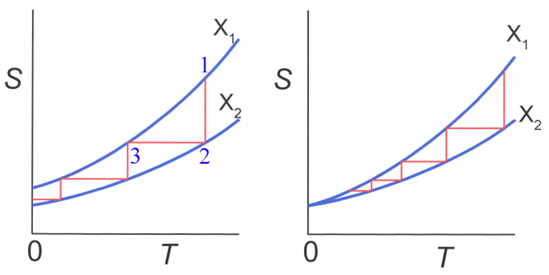
\includegraphics[width=\linewidth]{Lec6/magnetization.png}
%	\caption{Метод отримання наднизьких температур шляхом послідовних ізотермічного намагнічування і адіабатичного розмагнічування речовини}
%	\label{pic:magnetization}
%\end{figure}

\begin{figure}[!h]
	\centering
	\begin{subfigure}[l]{0.445\textwidth}
        % !TeX root = ../../test.tex


\begin{tikzpicture}[
  declare function={
    a=0.1;
    A=1.25;
    b=0.05;
    B=1;
    %
    g(\x)=a*\x^2 + A;
    f(\x)=b*\x^2 + B;
    %
    N(\x)=sqrt( (g(\x) - B)/b );  % <-- загальний вигляд
  },
    ultra thick
]

  % Графіки функцій
  \draw[red, samples=100, domain=0:6] plot ({\x}, {g(\x)});
  \draw[red, samples=100, domain=0:6] plot ({\x}, {f(\x)});

  % Параметри
  \def\xstart{0}
  \def\numSteps{3}

  % Початкове x
  \pgfmathsetmacro\x{\xstart}

  % Цикл для сходинок
  \foreach \i in {1,...,\numSteps} {
    \pgfmathsetmacro\yLow{f(\x)}
    \pgfmathsetmacro\yHigh{g(\x)}
    \pgfmathsetmacro\xNext{N(\x)}
    \pgfmathsetmacro\yNextHigh{g(\xNext)}

    % Вгору, вправо, вгору
    \draw[blue]
      (\x,\yHigh) coordinate (a\i) -- (\xNext,\yHigh) coordinate (b\i) -- ({\xNext}, {\yNextHigh}) coordinate (c\i);

    % Оновити x
    \global\let\x\xNext
  }

   \node[right] at (c3) {$1$};
    \node[above] at (c3) {$X_1$};
   \node[right] at (b3) {$2$};
    \node[below] at (b3) {$X_2$};
   \node[left] at (a3) {$3$};

  % Осі
  \draw[->, thick] (0,-0.5) -- (0,6) node[above] {$S$};
  \draw[->, thick] (-0.5,0) -- (6,0) node[right] {$T$};
  \node[below right] at (0,0) {$T>0$};

\end{tikzpicture}
		\caption{}
		\label{pic:6.1a}
	\end{subfigure}
	\begin{subfigure}[r]{0.475\textwidth}
        \input{Lec6/tikz/STb.tikz}
		\caption{}
		\label{pic:6.1b}
	\end{subfigure}
	\caption{Метод отримання наднизьких температур шляхом послідовних ізотермічного намагнічування і адіабатичного розмагнічування речовини.}
	\label{pic:magnetization}
\end{figure}

Для отримання наднизьких температур використовують магнітний метод охолодження деяких речовин (парамагнітних солей), робота якого ілюструється на рис. \ref{pic:6.2}. Якщо парамагнітну речовину намагнічувати ізотермічно, то поле виконує роботу по орієнтації магнітних моментів атомів парамагнетика. Це можна трактувати так: сам парамагнетик виконує від'ємну роботу при намагнічуванні (ділянки $1-2$ та $3-4$). Отже, при розмагнічуванні парамагнетик виконує додатну роботу. Якщо процес розмагнічування $2-3$ адіабатичний (на практиці це досягається швидким виключенням поля), то за першим законом робота виконується за рахунок зменшення внутрішньої енергії. Для парамагнетика внутрішня енергія $U\sim T^{4}$ і не залежить від $\mathcal{M}$, звідки випливає, що $\Delta T$ від'ємне --- має місце охолодження. Неважко вирахувати величину отриманого охолодження. Перший закон для парамагнетика записується так:
\begin{equation}\label{6.9}
	TdS = dU - \mathcal{H}d\mathcal{M}
\end{equation}
де узагальнена сила – $\mathcal{H}$, а узагальнена координата --- $\mathcal{M}$. Тоді $\Delta T = \lpdr{T}{\mathcal{H}}{S}\Delta \mathcal{H}$. Знайдемо $\lpdr{T}{\mathcal{H}}{S}$:
\begin{equation}\label{6.10}
	\lpdr{T}{\mathcal{H}}{S} = \jacobi{T,S}{\mathcal{H},S}\jacobi{-\mathcal{H},\mathcal{M}}{T,S} = \jacobi{\mathcal{M},\mathcal{H}}{\mathcal{H},S}\jacobi{\mathcal{H},T}{\mathcal{H},T}=-\dfrac{T}{C_{\mathcal{H}}}\lpdr{\mathcal{M}}{T}{\mathcal{H}}
\end{equation}

%---------------------------------------------------------
\begin{figure}[h!]\centering

% !TeX root = ../../test.tex


\begin{tikzpicture}[
  declare function={
    SH(\x) = -exp(-\x) + 2*\x + 0.1*\x^2;
  }
]



		\coordinate [] (0) at (0, 0) ;
		\coordinate [] (1) at (2.25, 4.25) ;
		\coordinate [] (2) at (5.5, 5) ;
		\coordinate [] (3) at (3, 3) ;
		\coordinate [] (4) at (5.5, 3.75) ;

        \node[right] at (2) {$H = 0$};
         \node[right] at (4) {$H \neq 0$};

		\draw [ultra thick, name path=A, smooth, plotred]  (0) to[in=-150, out=0, looseness=0.75] (1) to [in=185, out=30, looseness=0.50] (2);
		\draw [ultra thick, name path=B, smooth, plotred] (0) to[in=215, out=0, looseness=1.50] (3) to [in=-165, out=35, looseness=0.50] (4);

        \path[name path=L1] (1.7247, 0) -- ++(0, 6);
        \path[name path=L2] (5, 0) -- ++(0, 6);
        \path[name intersections={of=A and L1, name=I}] coordinate (A1) at (I-1);
        \path[name intersections={of=B and L1, name=I}] coordinate (B1) at (I-1);
        \path[name intersections={of=A and L2, name=I}] coordinate (A2) at (I-1);
        \path[name intersections={of=B and L2, name=I}] coordinate (B2) at (I-1);

        \draw[plotblue] (B1) -- node[above, sloped, inner sep=0.5pt, font=\scriptsize] {$\Delta S_\text{маг}$} node (IT) {} (A1) -- node[above, font=\scriptsize,inner sep=0.5pt] {$\Delta T_\text{ад}$} node (AD) {}   (B2) -- (A2);

        \node[circle, inner sep=1.5pt, fill] at (B1) {}; \node[right] at (B1) {$4$};
        \node[circle, inner sep=1.5pt, fill] at (A1) {}; \node[below right] at (A1) {$3$};
        \node[circle, inner sep=1.5pt, fill] at (B2) {}; \node[below] at (B2) {$2$};
        \node[circle, inner sep=1.5pt, fill] at (A2) {}; \node[above] at (A2) {$1$};

        \node[font=\scriptsize\sffamily] (AT) at (5, 1.5) {Адіабатичний процес};
        \node[font=\scriptsize\sffamily] (TT) at (5, 1) {Ізотермічний процес};

        \draw[->, ultra thick, cyan] (AT) to[out=90, in=270]  (AD.south west);
        \draw[->, ultra thick, cyan] (TT.west) to[out=180, in=0] (IT.east);


  % Осі
  \draw[->, thick] (0,-0.5) -- (0,6) node[above] {$S$};
  \draw[->, thick] (-0.5,0) -- (6,0) node[right] {$T$};
\end{tikzpicture}
\caption{Процес охолодження за рахунок почергового адіабатичного розмагнічування та ізотермічного намагнічування речовини.}
\label{pic:6.2}
\end{figure}
%---------------------------------------------------------


Зокрема для парамагнетика мають місце такі співвідношення для теплоємності і намагнетованості $C_{\mathcal{H}}=\alpha T^{3}$ та $\mathcal{M} = \xi \dfrac{\mathcal{H}}{T}$, відповідно, звідки із (\ref{6.10}) і (\ref{6.9}):
\begin{equation}\label{6.11}
	\Delta T = \dfrac{\xi}{\alpha}\dfrac{\mathcal{H}}{T}\Delta \mathcal{H}<0
\end{equation}
оскільки $\Delta \mathcal{H}<0$. Видно, що охолодження тим ефективніше, чим нижча температура, але лише до певної межі, доки виконується закон Кюрі-Вейса, використаний при виведенні \eqref{6.11}. Відповідно до закону парамагнітна сприятливість обернено пропорційна температурі:
\begin{equation}\label{6.12}
	\chi = \dfrac{\xi}{T}
\end{equation}
Тут $\chi=\lpdr{\mathcal{M}}{\mathcal{H}}{T}$ --- ізотермічна сприйнятливість. Тоді, із (\ref{6.12}) випливає, що $\mathcal{M} = \xi\dfrac{\mathcal{H}}{T}$, і $\lpdr{ \mathcal{M}}{T}{\mathcal{H}}=-\xi\dfrac{\mathcal{H}}{T^2}$. Отримане співвідношення дійсно працює до дуже низьких температур.

При наближені до абсолютного нуля температур навіть дуже слабкої взаємодії між магнітними моментами атомів достатньо, що вони розташовувалися в певному порядку, що мінімізує загальну енергію системи (рис.~\ref{pic:6.3}). Магнітне поле може визначити напрямок магнітних моментів, проте на степінь їх упорядкованості практично не впливає. Таким чином, при адіабатичному розмагнічуванні парамагнітних солей досягаються температури до $1m$K, а при використанні ефекту розмагнічування ядерних магнітних дипольних моментів --- до $1\mu$K.

%---------------------------------------------------------
\begin{figure}[h!]\centering
%
\includegraphics[width=0.5\linewidth]{Pic6.3MagneticMoments}
% !TeX root = ../../test.tex


\begin{tikzpicture}[]
        \pgfmathsetmacro\hl{0.25}

% Magnetic moments at T1 (higher temperature)
\foreach \x in {0,...,3}
    \foreach \y in {0,...,3} {
        \pgfmathsetmacro{\angle}{90 + rand*100}
            \draw[->, plotblue, thick]
              ({\x - \hl*cos(\angle)}, {\y - \hl*sin(\angle)})
                --
              ({\x + 1.5*\hl*cos(\angle)}, {\y + 1.5*\hl*sin(\angle)});
        \node[ball color=plotred, minimum size=0.25cm, circle, inner sep=0] at (\x, \y) {};
    }
\node[below] at (1.5,-0.6) {$T_1$};

%% Magnetic moments at T2 < T1 (lower temperature)
\begin{scope}[xshift=5cm]
\foreach \x in {0,...,3}
    \foreach \y in {0,...,3} {
        \pgfmathsetmacro{\angle}{90 + rand*60}
            \draw[->, plotblue, thick]
              ({\x - \hl*cos(\angle)}, {\y - \hl*sin(\angle)})
                --
              ({\x + 1.5*\hl*cos(\angle)}, {\y + 1.5*\hl*sin(\angle)});
        \node[ball color=plotred, minimum size=0.25cm, circle, inner sep=0] at (\x, \y) {};
    }
\node[below] at (1.5,-0.6) {$T_2 < T_1$};
\end{scope}
%
%% Magnetic moments at T → 0K (all aligned)
\begin{scope}[xshift=10cm]
\foreach \x in {0,...,3}
    \foreach \y in {0,...,3} {
        \pgfmathsetmacro{\angle}{90 + rand*10}
            \draw[->, plotblue, thick]
              ({\x - \hl*cos(\angle)}, {\y - \hl*sin(\angle)})
                --
              ({\x + 1.5*\hl*cos(\angle)}, {\y + 1.5*\hl*sin(\angle)});
        \node[ball color=plotred, minimum size=0.25cm, circle, inner sep=0] at (\x, \y) {};
    }
\node[below] at (1.5,-0.6) {$T\to0$ K};
\end{scope}

\end{tikzpicture}
\caption{Ступінь упорядкованості магнітних моментів речовини із наближенням до абсолютного нуля температур зростає і перестає залежати від прикладеного магнітного поля.}
\label{pic:6.3}
\end{figure}
%---------------------------------------------------------


Проте, згідно з третім законом похідна від намагнетованості від температури $\lpdr{\mathcal{M}}{T}{\mathcal{H}}$  як один із термодинамічних коефіцієнтів прямує до нуля при  $T\rightarrow0$,  а отже, із \eqref{6.10} виходить  $\lpdr{T}{\mathcal{H}}{S}\rightarrow0$. Таким чином, ілюстрацією до процесу отримання наднизьких температур шляхом адіабатичного охолодження радше є рис.~\ref{pic:6.1b}, що демонструє неможливість досягнення $T=0$ за кінцеву кількість кроків.